\documentclass[12pt,a4paper]{article}

% --- PAQUETES DE CONFIGURACIÓN FORMAL Y FUENTES (XeLaTeX) ---
\usepackage{fontspec}
\setmainfont{Arial}

\usepackage[spanish,es-noquoting]{babel}
\usepackage{amsmath,amssymb,amsfonts}
\usepackage{geometry}
\geometry{a4paper, margin=2.5cm}
\usepackage{setspace}
\onehalfspacing

\usepackage{graphicx}
\usepackage{xcolor}
\usepackage{booktabs}
\usepackage{caption}
\usepackage{subcaption}
\usepackage{float}
\usepackage{hyperref}
\usepackage{listings}

% --- CONFIGURACIÓN DE NORMAS APA Y ENLACES ---
\hypersetup{
    colorlinks=true,
    linkcolor=black,
    citecolor=black,
    urlcolor=blue
}

\lstset{
    language=Python,
    basicstyle=\ttfamily\small,
    keywordstyle=\color{blue},
    stringstyle=\color{red},
    commentstyle=\color{gray},
    breaklines=true,
    showstringspaces=false
}

\begin{document}

% ==============================================================================
% PORTADA FORMAL (No cuenta para el límite de 12 páginas)
% ==============================================================================
\begin{titlepage}
    \centering
    \vspace*{0.5cm}
    {\Large \textbf{UNIVERSIDAD NACIONAL DE SAN LUIS}}\\[0.3cm]
    {\large Facultad de Ciencias Físico Matemáticas y Naturales}\\[0.2cm]
    {\large Licenciatura en Análisis y Gestión de Datos}\\[1.2cm]
    
    {\Large \textbf{CÁLCULO II --- TPAG 2026}}\\[0.4cm]
    {\Large \textbf{INFORME FINAL DE APLICACIÓN GRUPAL}}\\[1.2cm]
    
    \rule{\textwidth}{1pt}\\[0.4cm]
    {\Large \textbf{Análisis Geométrico de la Frontera de Normalidad y Dinámica Multivariable del Error en el Plano de Componentes Principales ($V_1, V_2$) para la Detección de Fraude Financiero}}\\[0.2cm]
    \rule{\textwidth}{1pt}\\[1.5cm]
    
    \begin{flushleft}
    \textbf{Docente Responsable:} Mgtr. Ing. Martín Garciarena Ucelay\\[0.3cm]
    \textbf{Grupo N.º:} 2\\[0.3cm]
    \textbf{Integrantes:}\\[0.1cm]
    \begin{itemize}
        \item ADARO, Marcelo
        \item FUNES, Samanta Celeste
        \item GIL, Inés
        \item GUIÑAZÚ, Leandro Sebastián
        \item LEDEZMA, Ricardo Mariano
    \end{itemize}
    \textbf{Enlace al Video Expositivo (YouTube/Drive):} \url{https://drive.google.com/link-video-grupo2}
    \end{flushleft}
    
    \vfill
    {\large San Luis, Argentina \\ 12 de noviembre de 2026}
\end{titlepage}

\newpage

% ==============================================================================
% DECLARACIÓN ÉTICA E ÍNDICE (No cuentan para el límite de 12 páginas)
% ==============================================================================
\section*{Declaración sobre el uso de herramientas de Inteligencia Artificial}
En cumplimiento de la normativa del TPAG 2026, el Grupo N.º 2 declara que se utilizaron herramientas de IA generativa únicamente para la revisión de sintaxis en LaTeX, asistencia en la maquetación del documento, soporte en la depuración de scripts en Python y asistencia analítica en la revisión técnica de consistencia. Todos los planteos teóricos, resoluciones analíticas, parametrizaciones, cálculos de integrales, generación de visualizaciones y discusiones conceptuales provienen estrictamente del desarrollo efectuado por los integrantes sobre el dataset real auditado.

\vspace{0.5cm}

\tableofcontents
\newpage

% ==============================================================================
% SECCIÓN A: INTRODUCCIÓN Y MARCO TEÓRICO
% ==============================================================================
\section{Introducción, contexto del problema y marco teórico}

\subsection{Contexto Real y Planteamiento del Problema}
La detección de transacciones fraudulentas con tarjetas de crédito es un desafío estratégico en el sector bancario. La principal dificultad analítica reside en el desbalance de clases extremo: en un flujo transaccional habitual, las operaciones fraudulentas representan menos del $0{,}2\%$ del total. Los algoritmos supervisados tradicionales tienden a presentar alto sobreajuste hacia la clase mayoritaria. Por ello, el enfoque más robusto consiste en caracterizar rigurosamente la masa operativa legítima y definir una frontera geométrica de normalidad.

\subsection{Objetivos del Análisis}
\begin{itemize}
    \item \textbf{Objetivo General:} Desarrollar un modelo geométrico-analítico continuo mediante herramientas de Cálculo II en el plano de las componentes principales $V_1$ y $V_2$, delimitando una región de seguridad mediante la distancia estandarizada con covarianza diagonal.
    \item \textbf{Unidad 1 (Funciones Vectoriales):} Parametrizar la frontera elíptica de seguridad $\vec{r}(t)$ para el umbral $c = 5{,}991$, analizando la velocidad $\vec{v}(t)$, la aceleración $\vec{a}(t)$, la curvatura $\kappa(t)$ y la longitud de arco $L$.
    \item \textbf{Unidad 2 (Funciones de Varias Variables):} Formular la función de error estandarizado $E_d(V_1, V_2)$, caracterizar su gradiente $\nabla E_d$, evaluar la derivada direccional $D_{\vec{u}} E_d$ y clasificar el centroide como un mínimo global estricto mediante la matriz Hessiana.
    \item \textbf{Unidad 3 (Integrales Múltiples y Campos Vectoriales):} Calcular la masa de probabilidad gaussiana retenida mediante integración doble en coordenadas polares generalizadas y evaluar el flujo saliente de anomalía mediante la versión de divergencia del Teorema de Green.
\end{itemize}

\subsection{Origen de los Datos y Modelo Estadístico de Partida}
Se utilizó el dataset público \textit{Credit Card Fraud Detection} (ULB / Kaggle), compuesto por $284.807$ transacciones reales. Se seleccionaron las dos primeras componentes principales ($V_1, V_2$). Los parámetros estadísticos calculados sobre la población de transacciones legítimas ($Class = 0$, $N = 284.315$) se presentan en la Tabla \ref{tab:estadisticos}.

\begin{table}[H]
\centering
\caption{Parámetros estadísticos de las transacciones legítimas ($Class = 0$).}
\label{tab:estadisticos}
\begin{tabular}{lrr}
\toprule
\textbf{Parámetro Estadístico} & \textbf{Variable $V_1$} & \textbf{Variable $V_2$} \\
\midrule
Media ($\mu$) & $0{,}00825774$ & $-0{,}00627086$ \\
Desviación Estándar ($\sigma$) & $1{,}92981405$ & $1{,}63614605$ \\
Covarianza observada $\sigma_{12}$ & \multicolumn{2}{c}{$0{,}07100000$ (Correlación $r = 0{,}022487$)} \\
\bottomrule
\end{tabular}
\end{table}

\paragraph{Justificación del Modelo Diagonal:} Aunque la covarianza observada es $\sigma_{12} = 0{,}0710$, la correlación lineal es prácticamente nula ($r \approx 0{,}0225$). Por consiguiente, se adopta de manera explícita el modelo de **distancia estandarizada con covarianza diagonal** (o aproximación diagonal de Mahalanobis), despreciando el término cruzado $V_1 V_2$. Esto permite trabajar con curvas de nivel elípticas alineadas con los ejes coordenados de las componentes principales sin alterar el rigor matemático del análisis multivariable.

\begin{figure}[H]
\centering
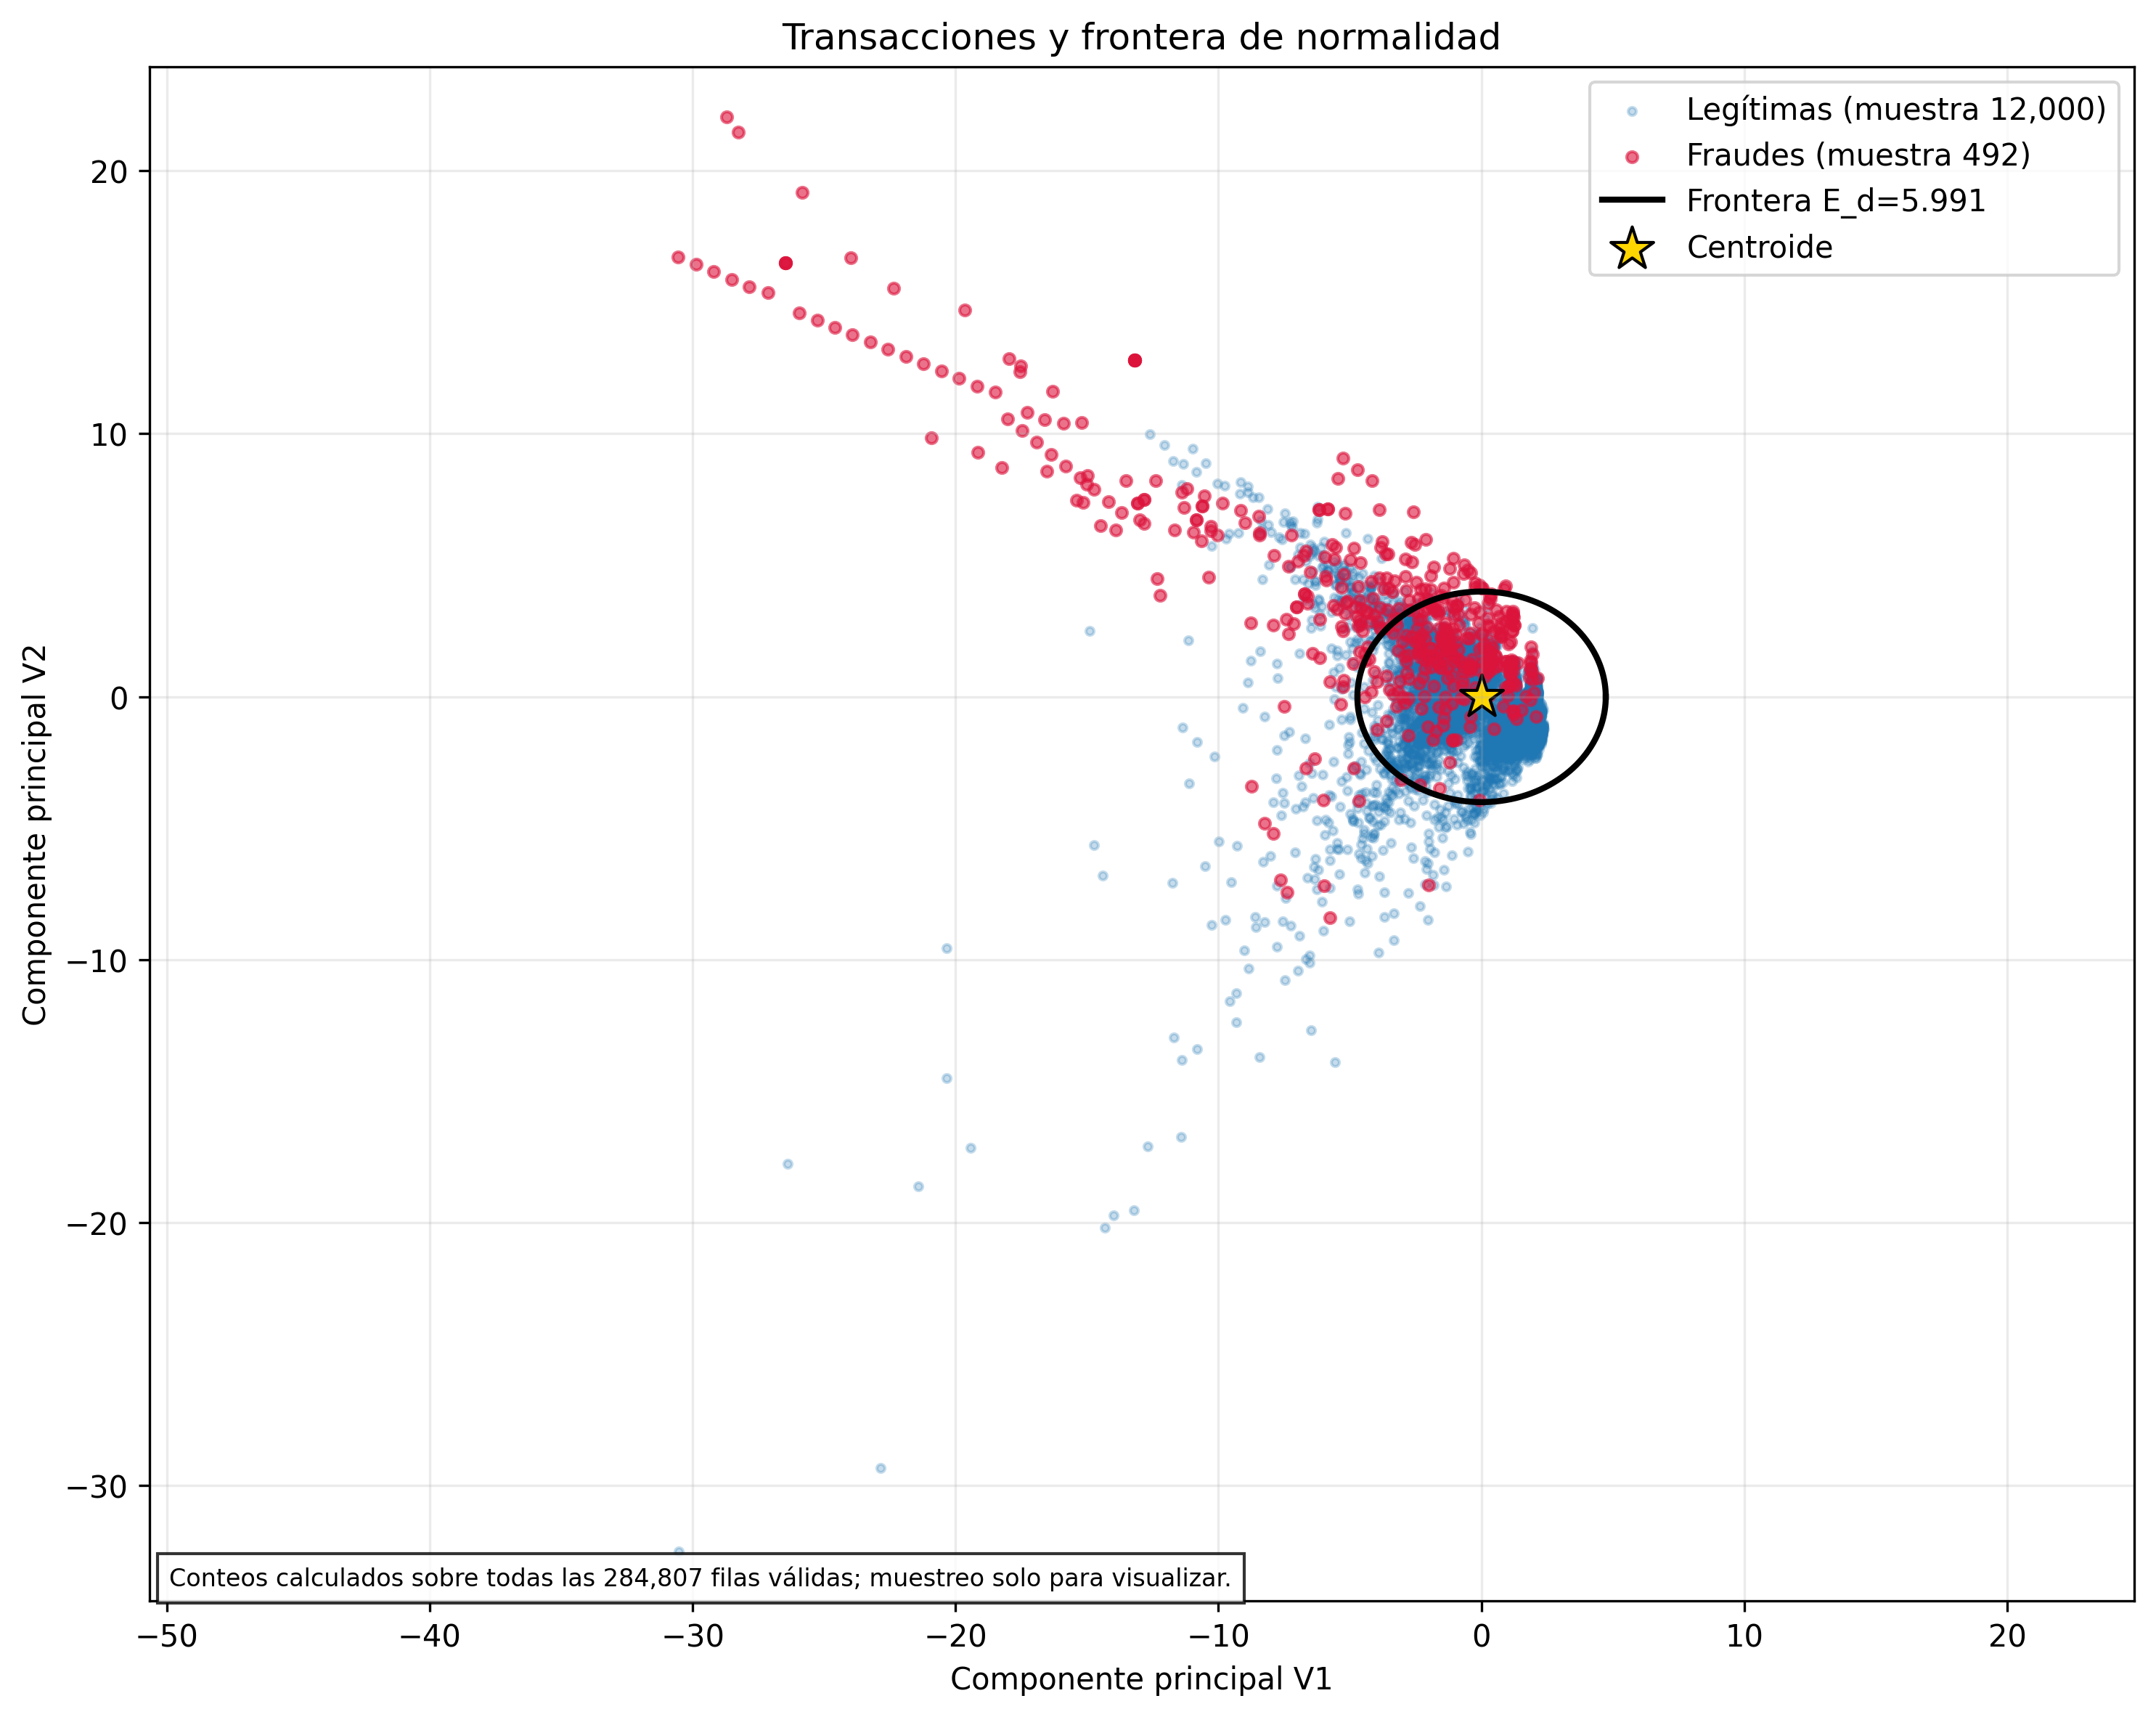
\includegraphics[width=0.85\textwidth]{grafico_1_datos_frontera.png}
\caption{Representación en el plano $V_1$-$V_2$ de la masa de transacciones legítimas y fraudulentas junto a la frontera elíptica de normalidad $E_d = 5{,}991$.}
\label{fig:dispersion_v1v2}
\end{figure}

\newpage

% ==============================================================================
% SECCIÓN B: FUNCIONES VECTORIALES (UNIDAD 1)
% ==============================================================================
\section{Funciones vectoriales y geometría de la frontera (Unidad 1)}

\subsection{Justificación de la Curva Elegida}
Para evitar conectar transacciones arbitrarias de distintos usuarios ordenadas en el tiempo (lo cual mediría ruido en lugar de un fenómeno dinámico), la función vectorial $\vec{r}(t)$ se define como la parametrización continua de la frontera elíptica $C = \partial R$ que delimita la región de normalidad $E_d(V_1, V_2) \le c$, con umbral $c = 5{,}991$ (percentil $95\%$ de la distribución $\chi^2$ con 2 grados de libertad).

\subsection{Parametrización de la Frontera Elíptica}
Con las desviaciones estándar $\sigma_1 = 1{,}929814$ y $\sigma_2 = 1{,}636146$, los semiejes de la elipse alineada son $a = \sigma_1 \sqrt{c} \approx 4{,}723513$ y $b = \sigma_2 \sqrt{c} \approx 4{,}004716$. La función vectorial parametrizada centrada en $\vec{\mu} = (\mu_1, \mu_2)$ es:
\begin{equation}
\vec{r}(t) = \langle 0{,}008258 + 4{,}723513 \cos(t), \; -0{,}006271 + 4{,}004716 \sin(t) \rangle, \quad t \in [0, 2\pi]
\end{equation}

\subsection{Cinemática: Velocidad, Rapidez y Aceleración}
Diferenciando componentes respecto del parámetro angular $t$:
\begin{equation}
\vec{v}(t) = \vec{r}'(t) = \langle -4{,}723513 \sin(t), \; 4{,}004716 \cos(t) \rangle
\end{equation}
La rapidez del recorrido angular sobre el contorno es:
\begin{equation}
\|\vec{v}(t)\| = \sqrt{22{,}311576 \sin^2(t) + 16{,}037751 \cos^2(t)}
\end{equation}
La aceleración vectorial apunta hacia el centroide de normalidad:
\begin{equation}
\vec{a}(t) = \vec{r}''(t) = \langle -4{,}723513 \cos(t), \; -4{,}004716 \sin(t) \rangle = -(\vec{r}(t) - \vec{\mu})
\end{equation}

\subsection{Curvatura Escalar Plana}
La curvatura plana $\kappa(t)$ de la frontera elíptica se calcula como:
\begin{equation}
\kappa(t) = \frac{|x'(t)y''(t) - y'(t)x''(t)|}{\|\vec{v}(t)\|^3} = \frac{a b}{(a^2 \sin^2(t) + b^2 \cos^2(t))^{3/2}}
\end{equation}
Evaluando en los vértices de la elipse:
\begin{itemize}
    \item Vértices del eje mayor ($t = 0, \pi$): $\kappa_{\max} = \frac{a}{b^2} = \frac{4{,}723513}{(4{,}004716)^2} \approx 0{,}294525$.
    \item Vértices del eje menor ($t = \frac{\pi}{2}, \frac{3\pi}{2}$): $\kappa_{\min} = \frac{b}{a^2} = \frac{4{,}004716}{(4{,}723513)^2} \approx 0{,}179491$.
\end{itemize}

\subsection{Longitud de Arco de la Frontera}
El perímetro total de la frontera de normalidad es la integral de la rapidez:
\begin{equation}
L = \int_{0}^{2\pi} \|\vec{v}(t)\| \, dt = \int_{0}^{2\pi} \sqrt{22{,}311576 \sin^2(t) + 16{,}037751 \cos^2(t)} \, dt
\end{equation}
Tratándose de una integral elíptica completa de segunda especie, se resolvió numricamente en Colab via `scipy.integrate.quad`, obteniéndose $L \approx 27{,}467052 \text{ unidades}$.

\begin{figure}[H]
\centering
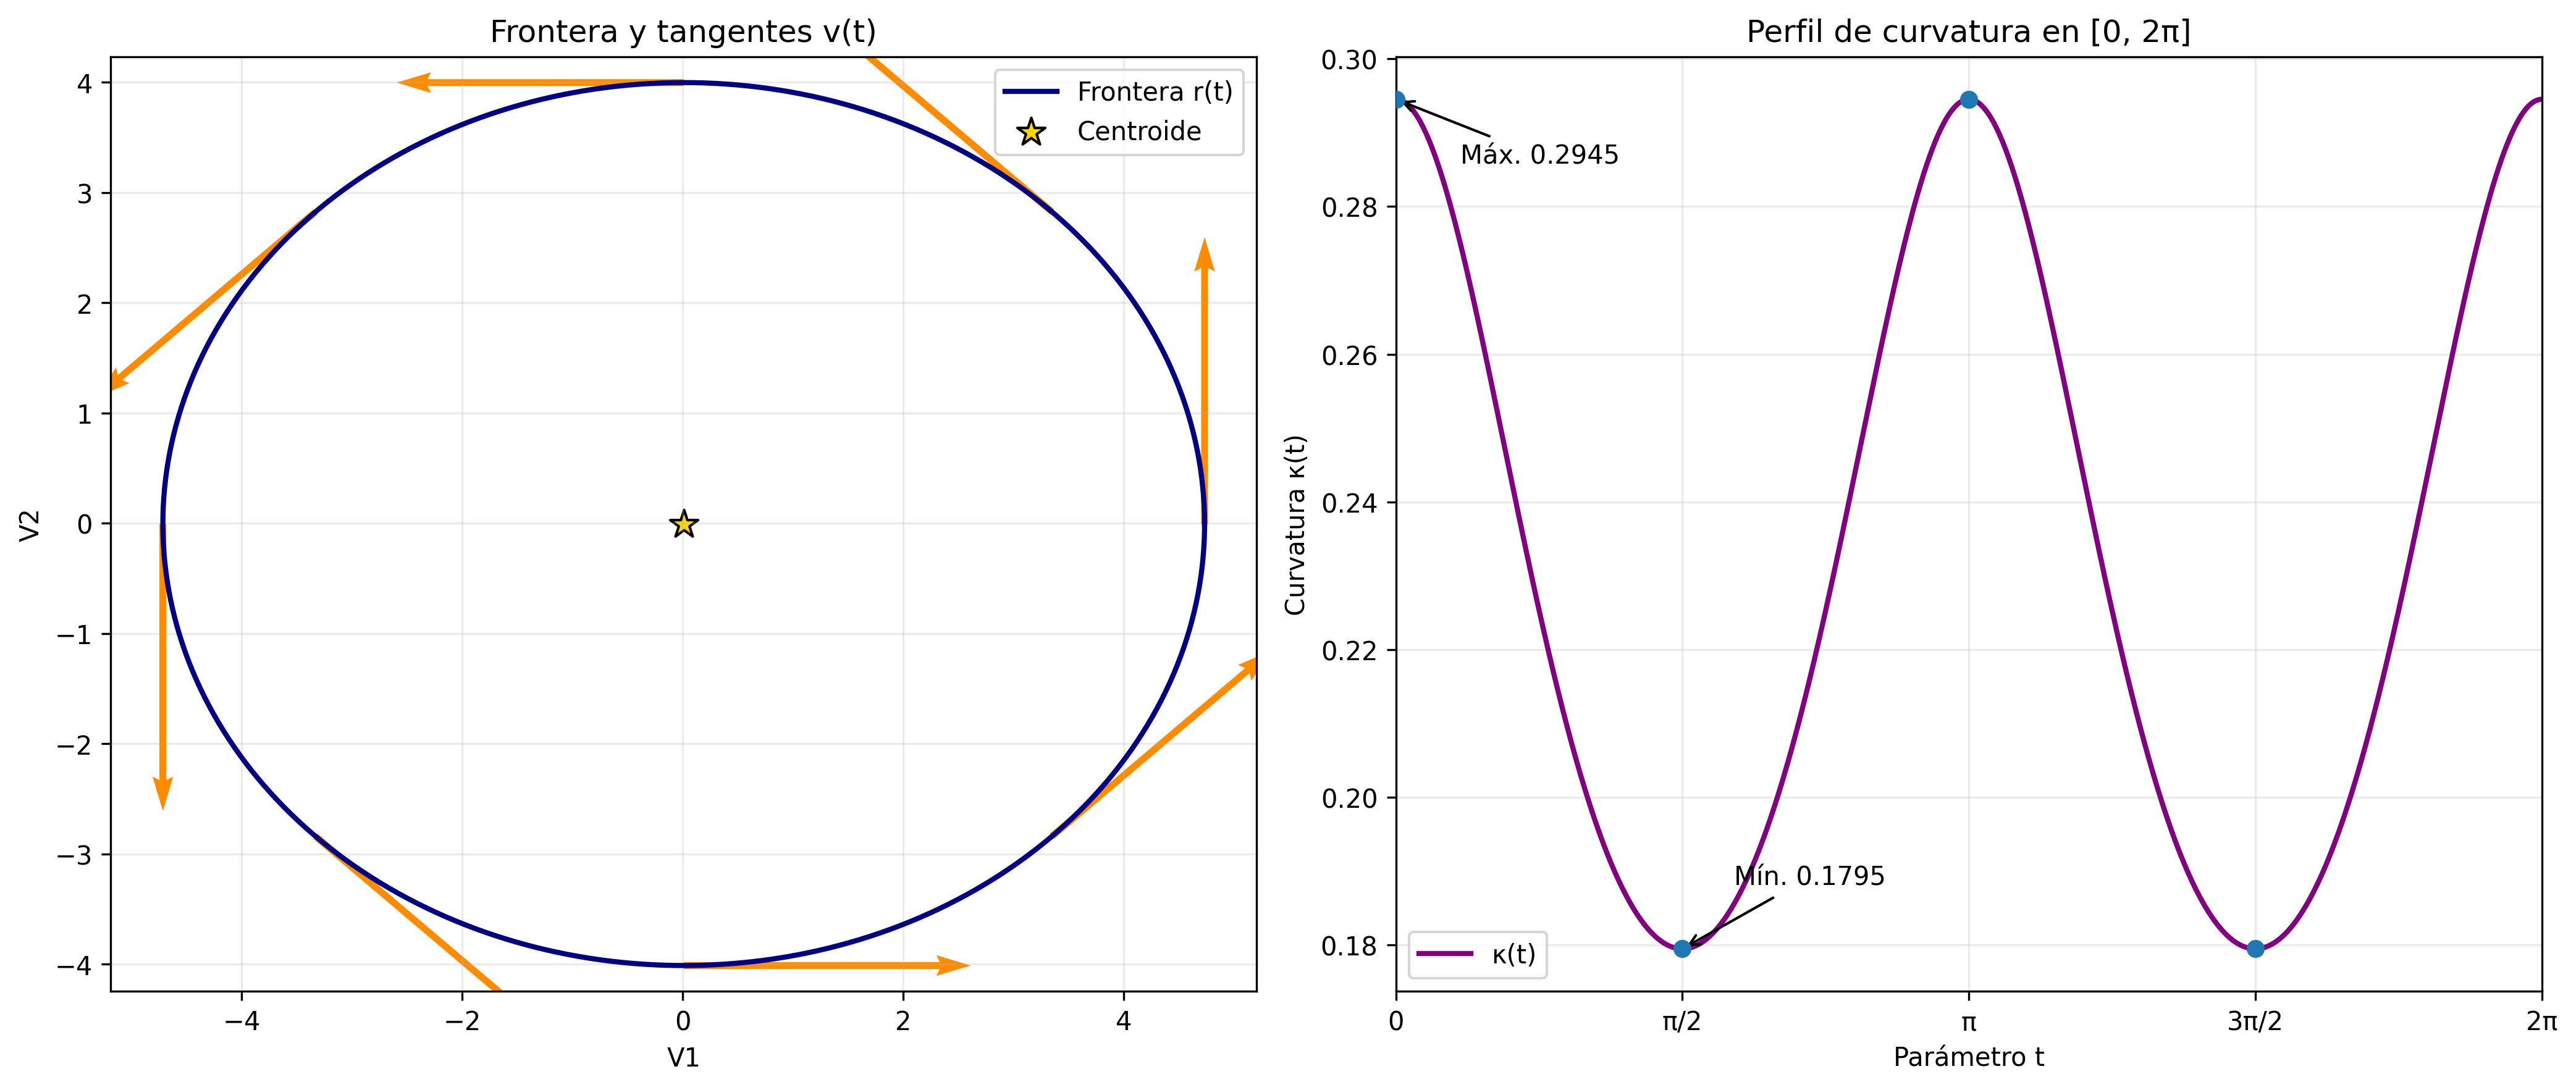
\includegraphics[width=0.9\textwidth]{grafico_2_curvatura_tangentes.png}
\caption{Frontera $r(t)$ con campo de vectores tangentes $\vec{v}(t)$ y perfil de curvatura escalar $\kappa(t)$.}
\label{fig:curvatura_tangentes}
\end{figure}

\newpage

% ==============================================================================
% SECCIÓN C: FUNCIONES DE VARIAS VARIABLES (UNIDAD 2)
% ==============================================================================
\section{Superficie de error, gradiente y optimización (Unidad 2)}

\subsection{Definición de la Función de Error Estandarizado}
Se define la función de error cuadrático estandarizado $E_d: \mathbb{R}^2 \to \mathbb{R}_{\ge 0}$ como la distancia adimensional respecto al centroide de las operaciones legítimas:
\begin{equation}
E_d(V_1, V_2) = \frac{(V_1 - \mu_1)^2}{\sigma_1^2} + \frac{(V_2 - \mu_2)^2}{\sigma_2^2} = \frac{(V_1 - 0{,}008258)^2}{3{,}724182} + \frac{(V_2 + 0{,}006271)^2}{2{,}676974}
\end{equation}

\subsection{Derivadas Parciales y Vector Gradiente}
Las derivadas parciales de primer orden representan las tasas instantáneas de incremento del puntaje de anomalía respecto de cada componente:
\begin{equation}
\frac{\partial E_d}{\partial V_1} = \frac{2(V_1 - \mu_1)}{\sigma_1^2} \approx 0{,}537038 (V_1 - 0{,}008258)
\end{equation}
\begin{equation}
\frac{\partial E_d}{\partial V_2} = \frac{2(V_2 - \mu_2)}{\sigma_2^2} \approx 0{,}747154 (V_2 + 0{,}006271)
\end{equation}
El vector gradiente $\nabla E_d(V_1, V_2) = \langle \frac{\partial E_d}{\partial V_1}, \frac{\partial E_d}{\partial V_2} \rangle$ señala la dirección de máxima tasa de aumento del riesgo y es ortogonal a las curvas de nivel elípticas $E_d(V_1, V_2) = k$.

\subsection{Derivada Direccional}
Para evaluar la tasa de cambio del puntaje en una dirección arbitraria dada por el vector unitario $\vec{u} = \langle u_1, u_2 \rangle$, aplicamos la propiedad del gradiente:
\begin{equation}
D_{\vec{u}} E_d(V_1, V_2) = \nabla E_d(V_1, V_2) \cdot \vec{u} = \frac{2(V_1 - \mu_1)}{\sigma_1^2} u_1 + \frac{2(V_2 - \mu_2)}{\sigma_2^2} u_2
\end{equation}
\paragraph{Ejemplo de Aplicación en la Frontera:} Evaluando en el vértice del eje mayor $\mathbf{P} = (\mu_1 + a, \mu_2) = (4{,}731771, -0{,}006271)$ en la dirección saliente radial $\vec{u} = \langle 1, 0 \rangle$:
\begin{equation}
D_{\vec{u}} E_d(\mathbf{P}) = \nabla E_d(\mathbf{P}) \cdot \langle 1, 0 \rangle = \left\langle \frac{2 a}{\sigma_1^2}, 0 \right\rangle \cdot \langle 1, 0 \rangle = \frac{2 \sqrt{c}}{\sigma_1} \approx 2{,}537233
\end{equation}
Este valor positivo cuantifica la velocidad con la que el indicador de anomalía se dispara al alejarse de la frontera de normalidad a lo largo del eje $V_1$.

\subsection{Puntos Críticos y Clasificación mediante la Matriz Hessiana}
Igualando el gradiente al vector nulo $\nabla E_d = \vec{0}$, obtenemos como único punto crítico el centroide $\mathbf{P}_c = (0{,}008258, -0{,}006271)$. Calculando las derivadas de segundo orden:
\begin{equation}
\frac{\partial^2 E_d}{\partial V_1^2} = \frac{2}{\sigma_1^2} \approx 0{,}537038, \quad \frac{\partial^2 E_d}{\partial V_2^2} = \frac{2}{\sigma_2^2} \approx 0{,}747154, \quad \frac{\partial^2 E_d}{\partial V_1 \partial V_2} = 0
\end{equation}
La matriz Hessiana $H(E_d)$ es constante y diagonal:
\begin{equation}
H(E_d) = \begin{pmatrix} 0{,}537038 & 0 \\ 0 & 0{,}747154 \end{pmatrix}
\end{equation}
El determinante de la matriz Hessiana (discriminante $D_H$) es:
\begin{equation}
D_H = \det(H) = (0{,}537038)(0{,}747154) - 0^2 \approx 0{,}401250 > 0
\end{equation}
Puesto que $D_H > 0$ y $\frac{\partial^2 E_d}{\partial V_1^2} > 0$, se demuestra analíticamente que $\mathbf{P}_c$ es un **mínimo local estricto**. Debido a que $H(E_d)$ es definida positiva en todo el plano $\mathbb{R}^2$, la superficie es estrictamente convexa y $\mathbf{P}_c$ constituye el **mínimo global absoluto**, con $E_d(\mathbf{P}_c) = 0$.

\begin{figure}[H]
\centering
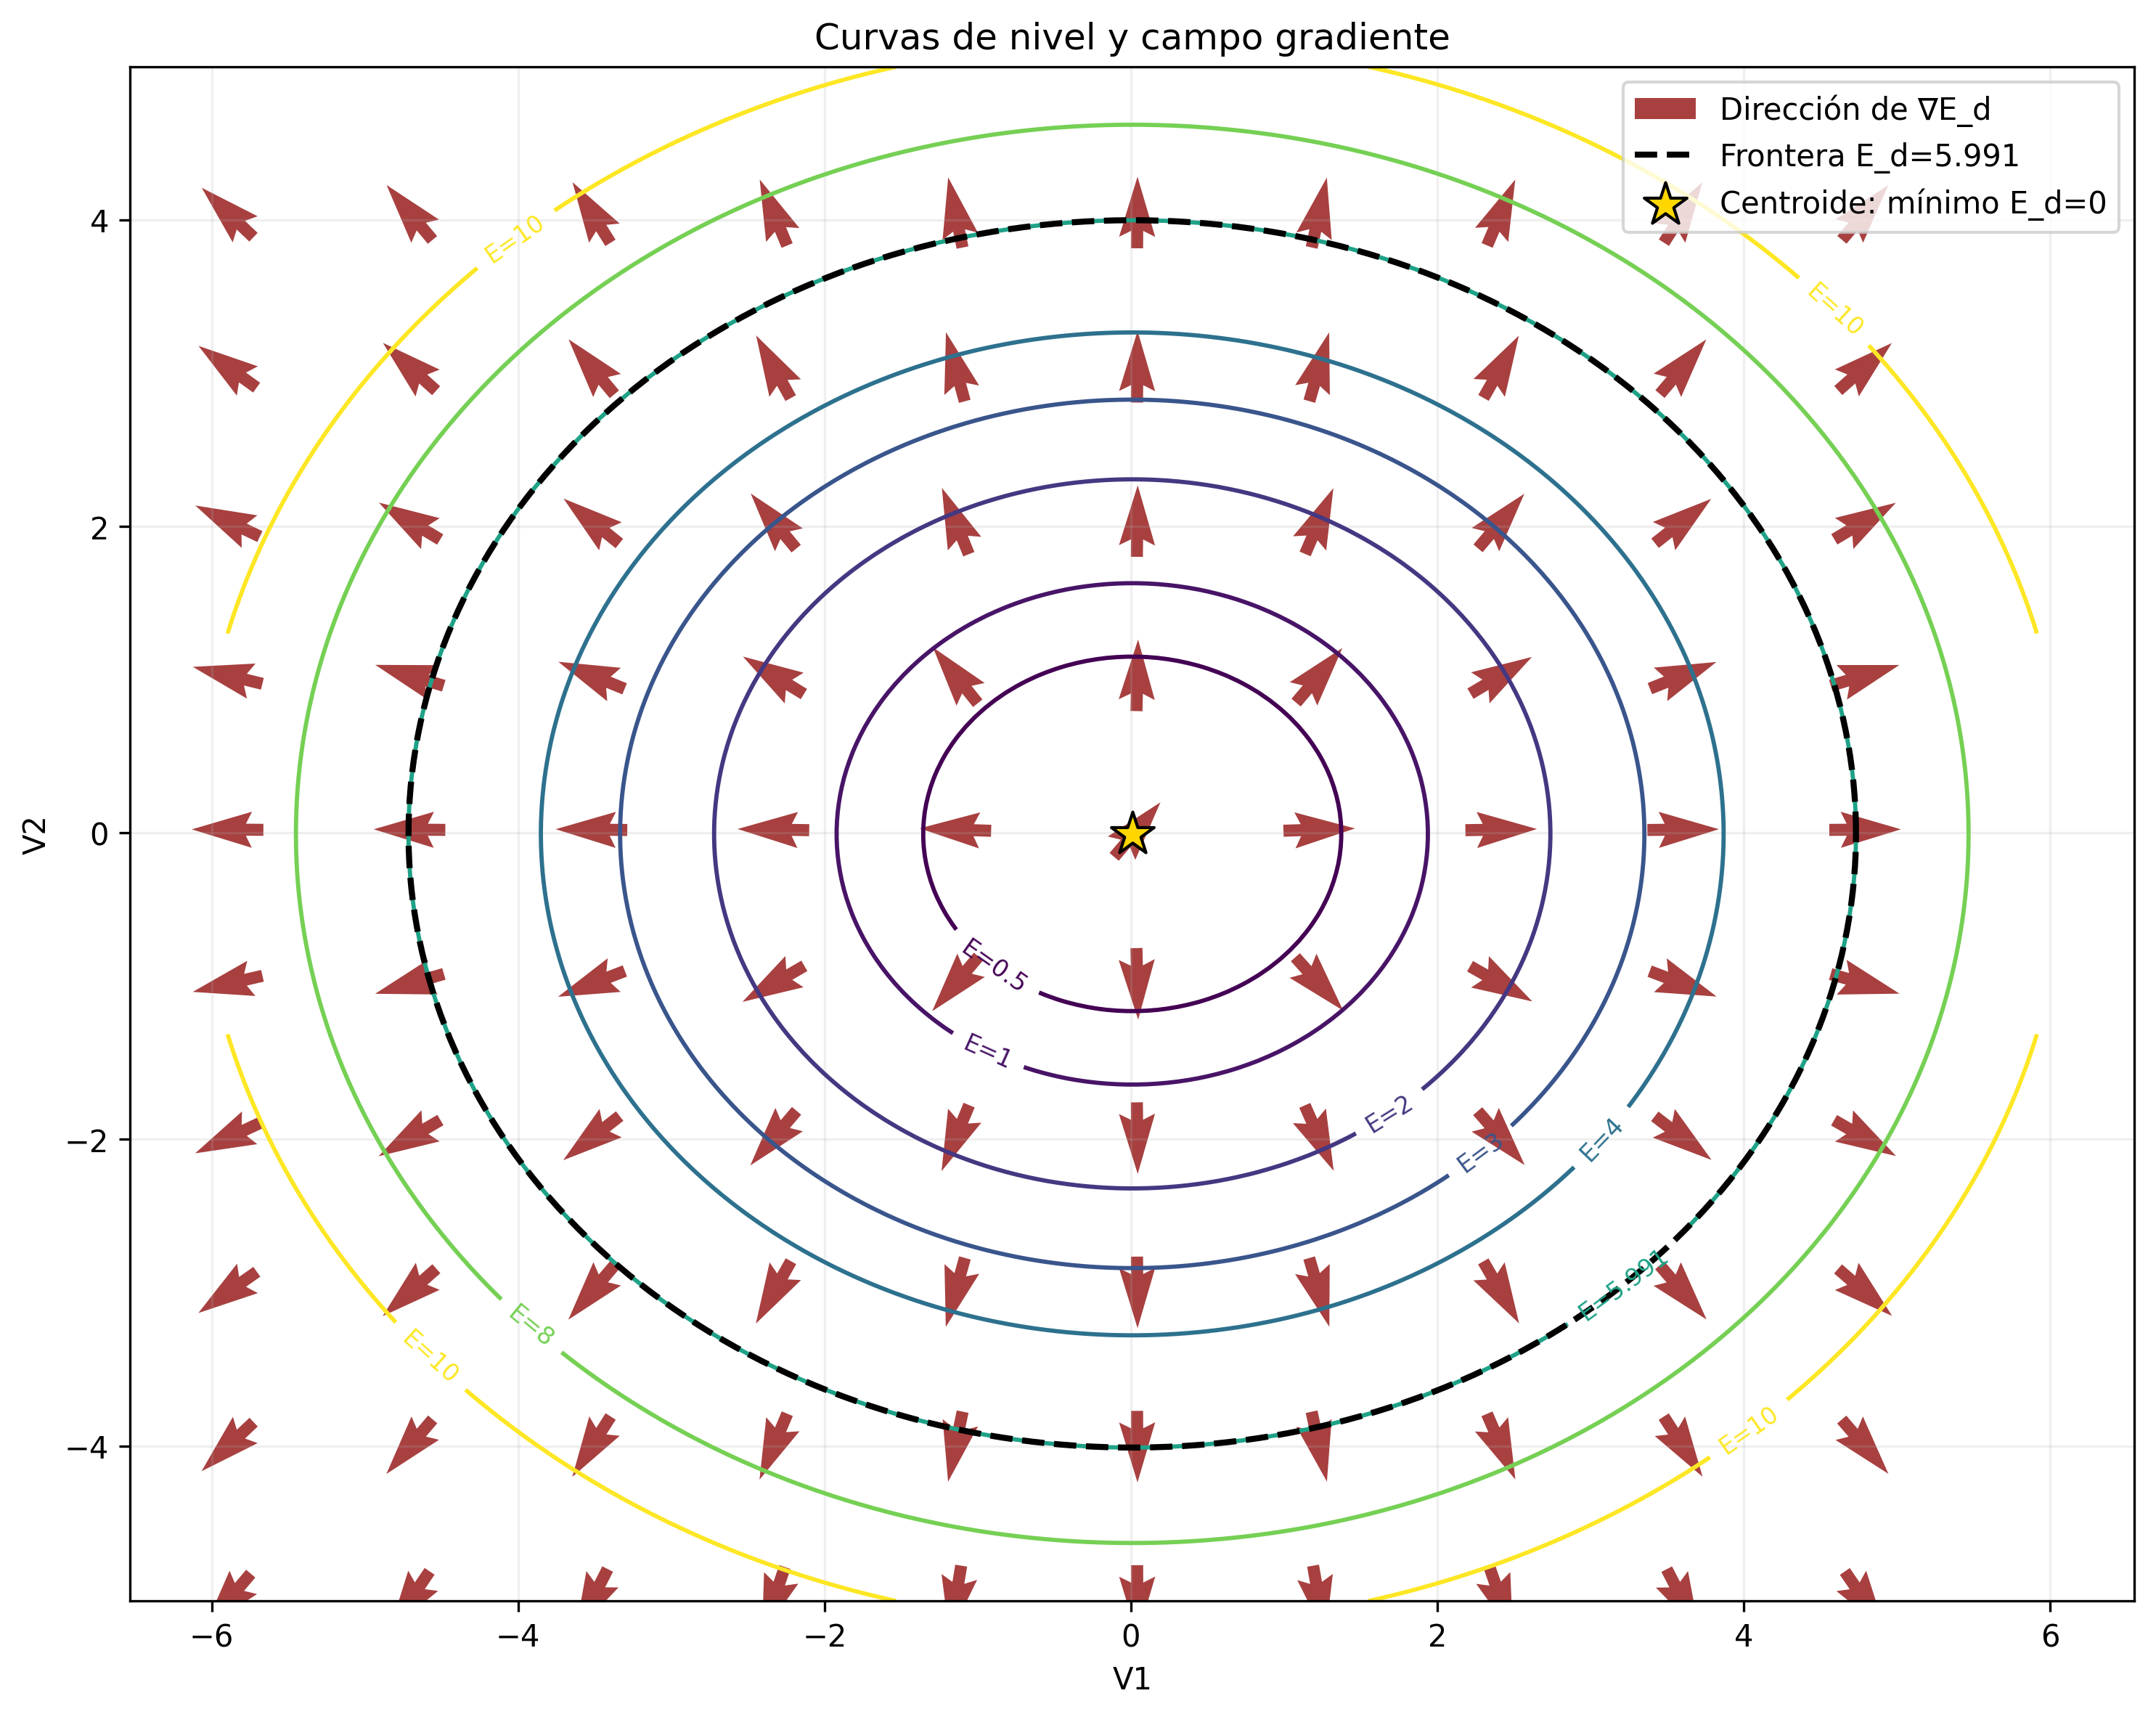
\includegraphics[width=0.85\textwidth]{grafico_3_niveles_gradiente.png}
\caption{Mapa de curvas de nivel elípticas de $E_d(V_1, V_2)$ y campo vectorial del gradiente $\nabla E_d$.}
\label{fig:niveles_gradiente}
\end{figure}

\newpage

% ==============================================================================
% SECCIÓN D: INTEGRALES MÚLTIPLES Y CAMPOS VECTORIALES (UNIDAD 3)
% ==============================================================================
\section{Integración doble, campos vectoriales y Teorema de Green (Unidad 3)}

\subsection{Masa de Probabilidad mediante Integración Doble}
Asumiendo la distribución normal bivariada ajustada para las operaciones legítimas, la densidad conjunta es:
\begin{equation}
\rho(V_1, V_2) = \frac{1}{2\pi \sigma_1 \sigma_2} \exp\left( -\frac{1}{2} E_d(V_1, V_2) \right)
\end{equation}
Para calcular la masa teórica retenida $M$ en la región elíptica $R = \{(V_1, V_2) \mid E_d(V_1, V_2) \le 5{,}991\}$, se aplica la transformación a **coordenadas polares generalizadas**:
\begin{equation}
V_1 = \mu_1 + \sigma_1 r \cos(\theta), \quad V_2 = \mu_2 + \sigma_2 r \sin(\theta)
\end{equation}
El Jacobiano de la transformación resulta:
\begin{equation}
J(r, \theta) = \left| \frac{\partial(V_1, V_2)}{\partial(r, \theta)} \right| = \begin{vmatrix} \sigma_1 \cos\theta & -\sigma_1 r \sin\theta \\ \sigma_2 \sin\theta & \sigma_2 r \cos\theta \end{vmatrix} = \sigma_1 \sigma_2 r
\end{equation}
Sustituyendo en la integral doble sobre la región transformada $R' = \{ (r, \theta) \mid 0 \le r \le \sqrt{c}, \, 0 \le \theta \le 2\pi \}$:
\begin{equation}
M = \int_{0}^{2\pi} \int_{0}^{\sqrt{5{,}991}} \frac{1}{2\pi \sigma_1 \sigma_2} e^{-r^2 / 2} (\sigma_1 \sigma_2 r) \, dr \, d\theta = \left( \frac{1}{2\pi} \int_{0}^{2\pi} d\theta \right) \left( \int_{0}^{\sqrt{5{,}991}} e^{-r^2 / 2} r \, dr \right)
\end{equation}
\begin{equation}
M = 1 \cdot \left[ -e^{-r^2 / 2} \right]_{0}^{\sqrt{5{,}991}} = 1 - e^{-5{,}991 / 2} = 1 - e^{-2{,}9955} \approx 0{,}949988 \quad (95{,}00\%)
\end{equation}

\subsection{Teorema de Green: Forma de Flujo de Anomalía}
Considerando el campo vectorial de anomalía $\vec{F}(V_1, V_2) = \nabla E_d$, evaluamos su flujo saliente $\Phi$ sobre la frontera elíptica orientada positivamente $C = \partial R$ mediante la **forma de flujo del Teorema de Green** (Teorema de la Divergencia en el plano):
\begin{equation}
\Phi = \oint_C \vec{F} \cdot \vec{n} \, ds = \iint_R (\nabla \cdot \vec{F}) \, dA
\end{equation}
La divergencia del campo gradiente equivale al Laplaciano de la función de error estandarizado:
\begin{equation}
\nabla \cdot \vec{F} = \Delta E_d = \frac{\partial^2 E_d}{\partial V_1^2} + \frac{\partial^2 E_d}{\partial V_2^2} = \frac{2}{\sigma_1^2} + \frac{2}{\sigma_2^2} \approx 0{,}537038 + 0{,}747154 = 1{,}284143
\end{equation}
Dado que la divergencia es constante en todo el plano, la integral doble se simplifica al producto de la divergencia por el área de la elipse $R$:
\begin{equation}
\text{Área}(R) = \pi a b = \pi (4{,}723513)(4{,}004716) \approx 59{,}427399 \text{ unidades}^2
\end{equation}
Por lo tanto, el flujo neto saliente a través del contorno es:
\begin{equation}
\Phi = (\nabla \cdot \vec{F}) \times \text{Área}(R) = 1{,}284143 \times 59{,}427399 \approx 76{,}313273
\end{equation}
Este resultado analítico coincide exactamente con el cálculo por integral de línea de contorno ejecutado en Python, verificando el Teorema de Green en el plano.

\begin{figure}[H]
\centering
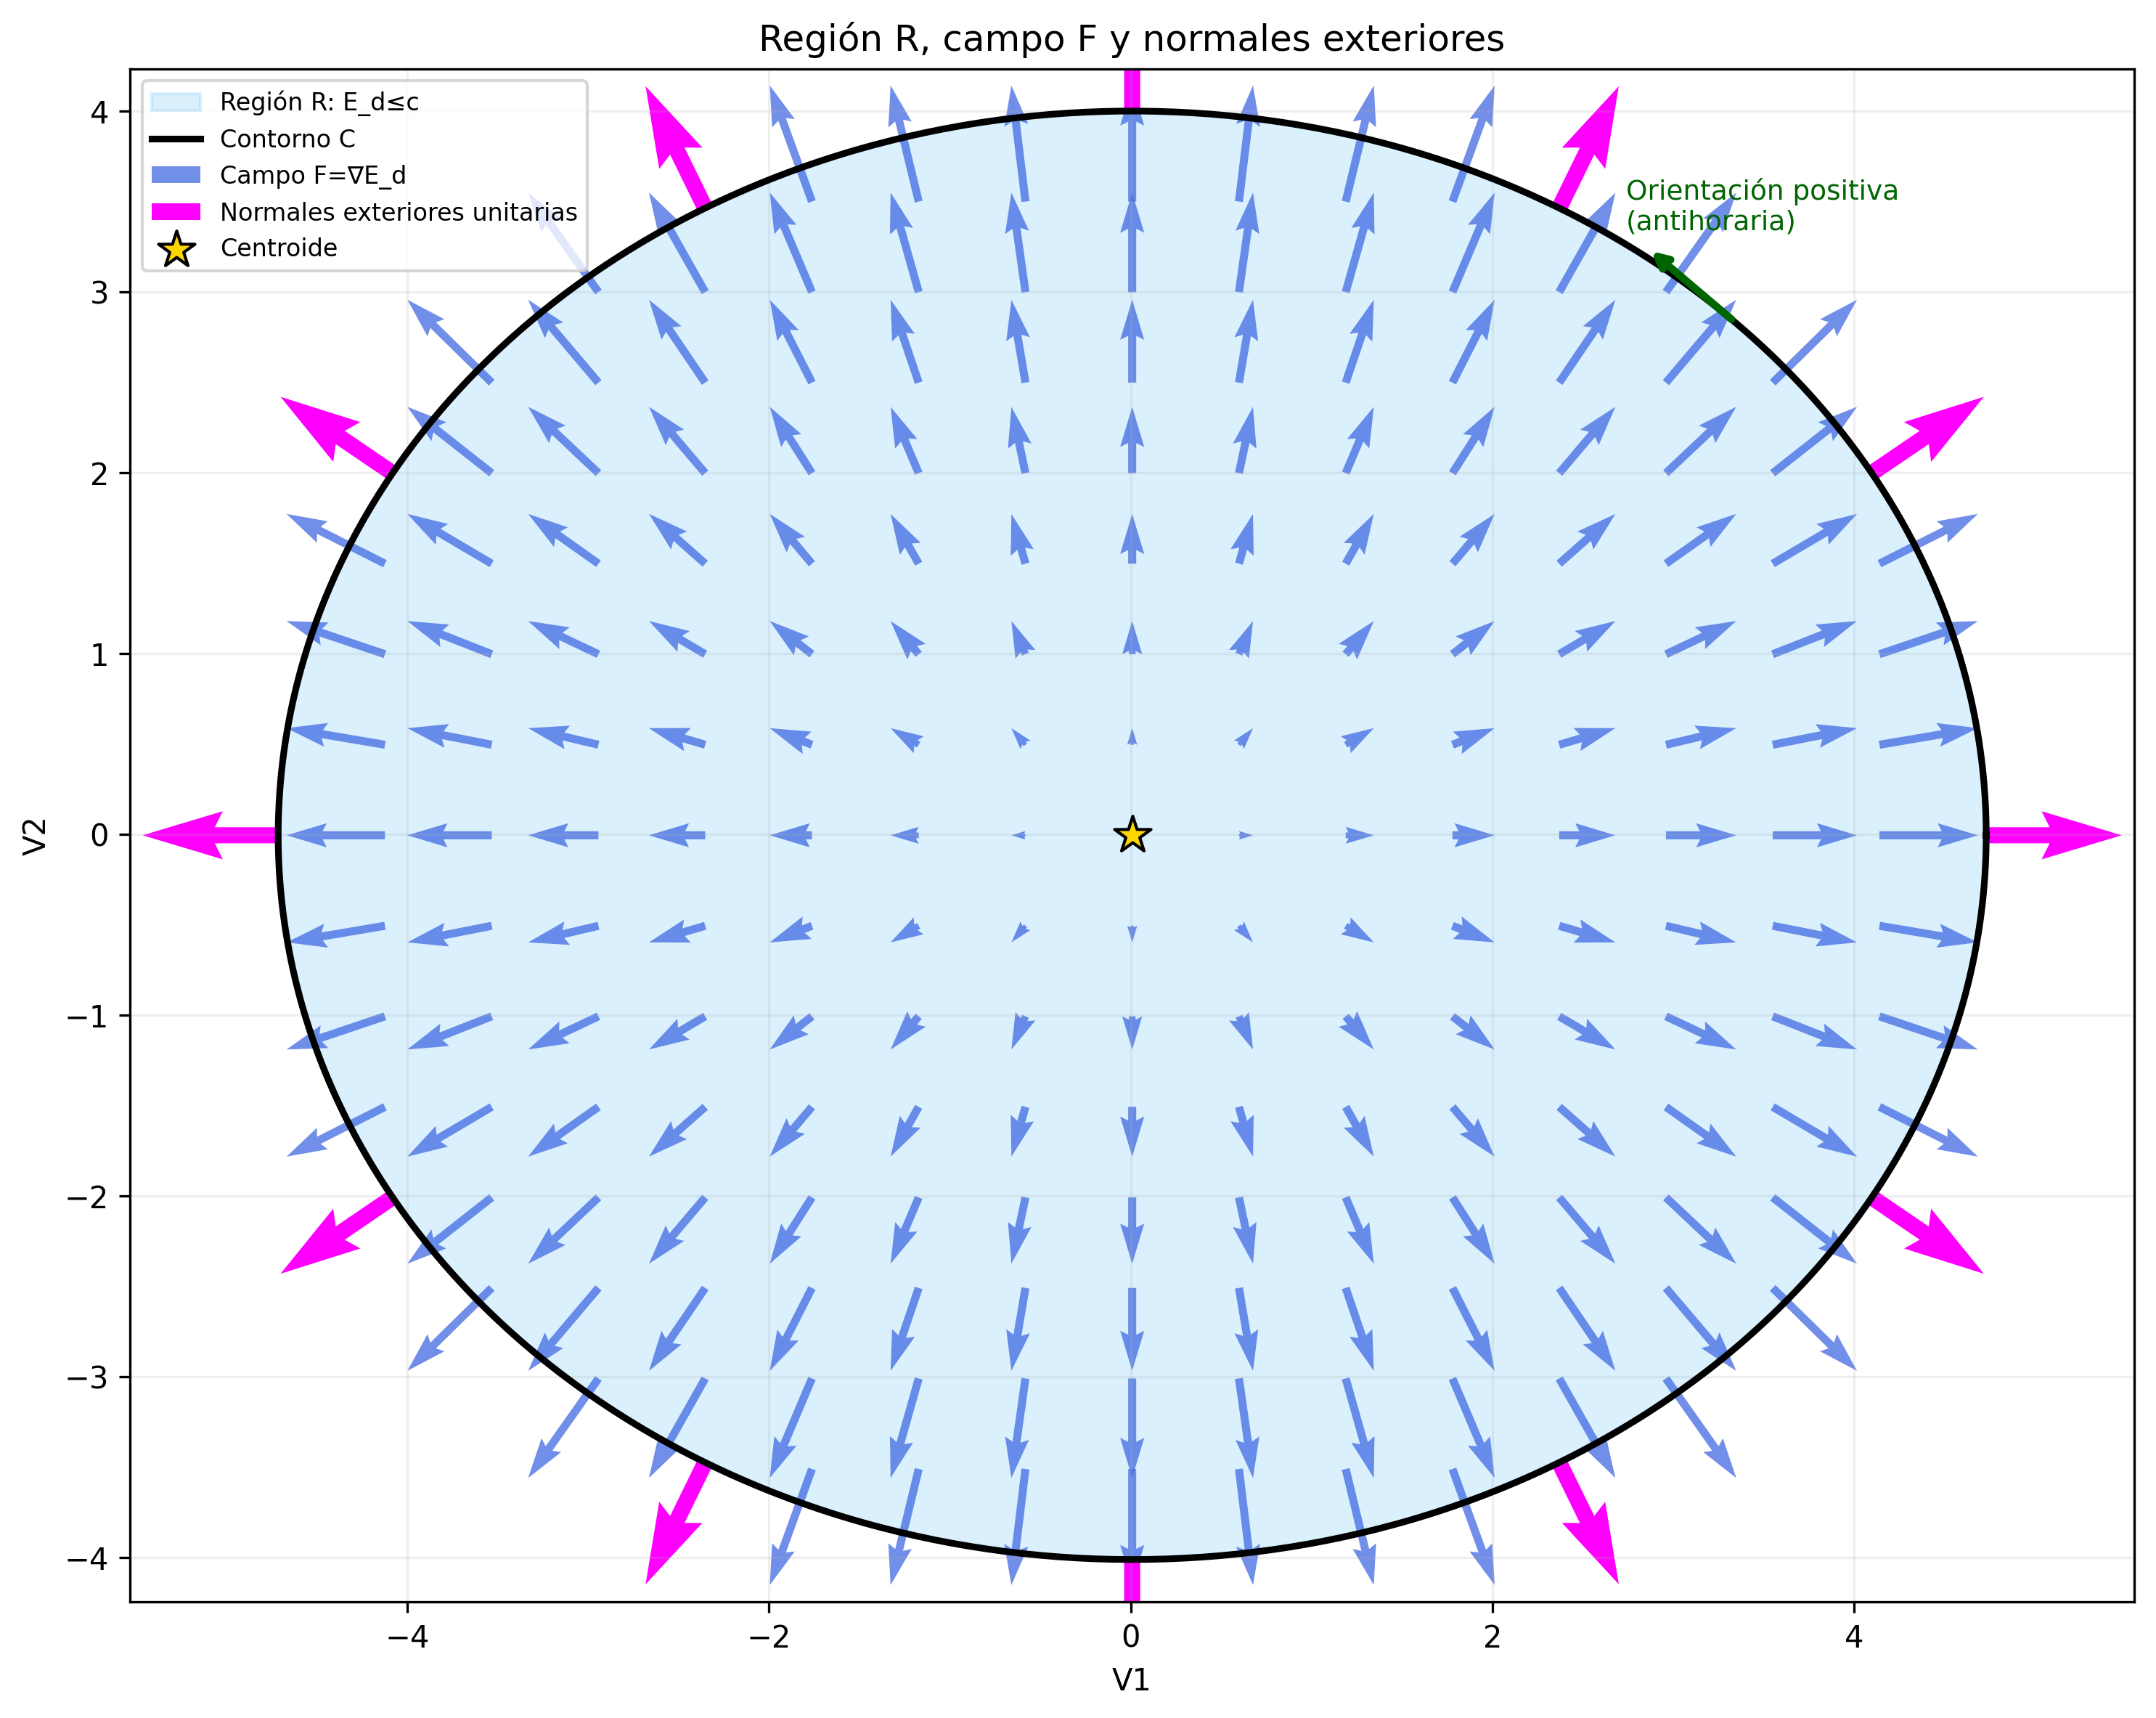
\includegraphics[width=0.85\textwidth]{grafico_4_region_flujo_normales.png}
\caption{Región de integración $R$, campo de anomalía $\vec{F} = \nabla E_d$ y vectores normales exteriores unitarios $\vec{n}$.}
\label{fig:region_flujo_normales}
\end{figure}

\newpage

% ==============================================================================
% SECCIÓN E: ANÁLISIS E INTERPRETACIÓN DE RESULTADOS
% ==============================================================================
\section{Análisis e interpretación de resultados}

\subsection{Evaluación Empírica sobre el Dataset Completo}
Al aplicar la regla de decisión $E_d(V_1, V_2) \le 5{,}991$ sobre la totalidad de las $284.807$ filas válidas del dataset, se obtuvo la matriz de confusión reportada en la Tabla \ref{tab:clasificacion}.

\begin{table}[H]
\centering
\caption{Resultados de clasificación del modelo sobre el dataset de Kaggle.}
\label{tab:clasificacion}
\begin{tabular}{lrrr}
\toprule
\textbf{Categoría} & \textbf{Dentro ($E_d \le 5{,}991$)} & \textbf{Fuera ($E_d > 5{,}991$)} & \textbf{Total Filas} \\
\midrule
Legítimas ($Class = 0$) & $272.572$ ($95{,}87\%$) & $11.743$ ($4{,}13\%$) & $284.315$ \\
Fraudes ($Class = 1$) & $258$ ($52{,}44\%$) & $234$ ($47{,}56\%$) & $492$ \\
\midrule
\textbf{Total} & $272.830$ & $11.977$ & $284.807$ \\
\bottomrule
\end{tabular}
\end{table}

\subsection{Métricas de Evaluación Bancaria}
A partir de los conteos observados ($TP = 234$, $FP = 11.743$, $TN = 272.572$, $FN = 258$), se desprenden las siguientes métricas de rendimiento:
\begin{itemize}
    \item \textbf{Sensibilidad / Cobertura de Fraude (Recall):} $\frac{TP}{TP + FN} = \frac{234}{492} \approx 47{,}5610\%$.
    \item \textbf{Especificidad:} $\frac{TN}{TN + FP} = \frac{272.572}{284.315} \approx 95{,}8697\%$.
    \item \textbf{Tasa de Falsos Positivos (FPR):} $\frac{FP}{TN + FP} = \frac{11.743}{284.315} \approx 4{,}1303\%$.
    \item \textbf{Precisión / Valor Predictivo Positivo (PPV):} $\frac{TP}{TP + FP} = \frac{234}{11.977} \approx 1{,}9537\%$.
    \item \textbf{Puntaje $F_1$:} $\frac{2 \cdot \text{Precisión} \cdot \text{Recall}}{\text{Precisión} + \text{Recall}} \approx 3{,}7554\%$.
\end{itemize}

\subsection{Discusión de Limitaciones y Valor Operativo}
1. \textbf{Filtro Exploratorio vs. Clasificador Final:} La precisión es de $1{,}95\%$, lo que implica que el $98{,}05\%$ de las alertas fuera de la elipse son transacciones legítimas inusuales. El modelo actúa como un **filtro exploratorio de primer nivel** en 2D, no como un bloqueador automático.
2. \textbf{Proyección Bidimensional:} Se utilizan únicamente 2 de las 28 componentes principales. El $52{,}44\%$ de los fraudes no detectados poseen comportamientos en $V_1$ y $V_2$ idénticos a las compras normales, requiriendo dimensiones superiores para su separación.

\newpage

% ==============================================================================
% SECCIÓN F: CONCLUSIONES Y PROPUESTAS DE MEJORA
% ==============================================================================
\section{Conclusiones y propuestas de mejora}

\subsection{Síntesis del Trabajo Integrador}
1. Se cumplieron satisfactoriamente todos los objetivos generales y específicos exigidos en las tres unidades de Cálculo II aplicados a un problema real de Data Science.
2. Se caracterizó analíticamente el centroide como el único mínimo global estricto mediante derivadas parciales y la matriz Hessiana.
3. Se parametrizó la frontera elíptica de normalidad mediante la función vectorial $\vec{r}(t)$, obteniendo su curvatura y su longitud de arco de $27{,}4671 \text{ unidades}$.
4. Se verificó la masa teórica ($95{,}00\%$) mediante integración doble en coordenadas polares generalizadas y se demostró la forma de flujo del Teorema de Green ($\Phi \approx 76{,}3133$).

\subsection{Propuestas de Mejora}
\begin{itemize}
    \item Extender la función de error a un espacio tridimensional $(V_1, V_2, V_3)$ o $n$-dimensional mediante la formulación matricial completa de Mahalanobis.
    \item Incorporar modelos no elípticos mediante estimación de densidad por núcleos (KDE) para adaptar la frontera a la asimetría real de los datos.
\end{itemize}

\newpage

% ==============================================================================
% SECCIÓN G: REFERENCIAS Y ANEXOS (Fuera del límite de 12 páginas)
% ==============================================================================
\section{Referencias y fuentes de datos}

\begin{itemize}
    \item Machine Learning Group --- ULB. (2013). \textit{Credit Card Fraud Detection Dataset} [Conjunto de datos]. Kaggle. \url{https://www.kaggle.com/datasets/mlg-ulb/creditcardfraud}
    \item Stewart, J. (2012). \textit{Cálculo de varias variables: Trascendentes tempranas} (7.ª ed.). Cengage Learning.
    \item Thomas, G. B. (2015). \textit{Cálculo: Varias variables} (13.ª ed.). Pearson Educación.
\end{itemize}

\end{document}
